\chapter{Technologien}
\label{ch:technical}

Für die Entwicklung eines Softwaresystems ist insbesondere bei der Implementierung entscheidend, welche Technologien verwendet werden.
Aus diesem Grund widmet sich diese Kapitel werden die technischen Aspekte der Plattform beschrieben.
Dabei werden die Technologien und Frameworks vorgestellt, die für die Entwicklung der Plattform verwendet wurden.

Die Plattform wurde mit den folgenden Technologien und Frameworks entwickelt:
\begin{itemize}
  \item \textbf{TypeScript} als Programmiersprache
  \item \textbf{React} als Frontend-Framework
  \item \textbf{\gls{mui}} als UI-Framework
  \item \textbf{Firebase} als Backend as a Service (\gls{baas})Plattform
  \item \textbf{Vercel} als Hosting-Plattform
  \item \textbf{Github} als Versionsverwaltungs-Plattform
  \item \textbf{Jira} als Projektmanagement-Plattform
\end{itemize}

Diese werden im Folgenden kurz vorgestellt.

\section{Grundlage für Technologieentscheidung}
\label{sec:technicalDecision}

Die einzige aus der Aufgabenstellung ersichtliche Vorgabe ist, dass das Softwareprodukt „Digital Hometown“ eine Plattform für den Austausch bieten soll.
Die Wahl der Technologie ist uns hierbei offengelassen.
Was daraus jedoch hervorgeht ist, dass es sich um eine für möglichst viele Nutzer verwendbare Web- oder Mobilanwendung handeln soll.
Insbesondere bei der Wahl einer Webanwendung, die dem Nutzer jeglichen Installationsaufwand erspart, ist die Hemmschwelle sehr gering, ein Softwareprodukt auszuprobieren.

Da, wie beschrieben, für eine solche Plattform des sozialen Austauschs eine ausreichend große Nutzerzahl entscheidend ist, fiel die Entscheidung schnell auf eine Webanwendung.
Obwohl beim aktuellen Stand der Plattform „Digital Dahoam“ nicht in erster Linie auf die Benutzbarkeit auf mobilen Endgeräten gelegt wurde, sei an dieser Stelle erwähnt, dass sich Webanwendungen mit etwas mehr Aufwand sehr gut auch für mobile Geräte wie Smartphones oder Tablets entwickeln lassen.
Der Fachbegriff hierfür ist die Umsetzung einer „Progressive Web-App“.

\section{TypeScript}
\label{sec:typescript}

TypeScript ist eine Erweiterung von Javascript, die statische Typisierung und Klassen hinzufügt.
Dadurch wird die Entwicklung von Software vereinfacht, da die Typisierung die Lesbarkeit des Codes verbessert und die Klassen die Wiederverwendbarkeit von Code ermöglichen.
Die Programmiersprache wird von Microsoft entwickelt und ist Open Source.\footnote{Vgl. TypeScript 2022 \cite{typescript2022}}

\subsection{Einsatz im Projekt}
\label{sub:typescriptUsage}

TypeScript wurde im Projekt verwendet, um die Entwicklung der Plattform zu vereinfachen. Der komplette Code der Website wurde mit TypeScript, HTML und CSS geschrieben, wobei TypeScript hierbei die Hauptrolle spielt.

\subsection{Grund für Technologieentscheidung}
\label{sub:typescriptReason}

Da TypeScript in großen Teilen der Javawelt inzwischen als de facto Standard ist um vor allem große Anwendungen sicher und effizient zu entwickeln, wurde diese Technologie für die Entwicklung der Plattform verwendet.
React (\ref{sec:react}), das größte Frontend-Framework der Welt, wird inzwischen auch in TypeScript entwickelt.\footnote{Vgl. TypeScript 2023 \cite{typescript2023}}

\section{React}
\label{sec:react}

React ist ein Open-Source Frontend-Framework, das von Facebook entwickelt wird.
Es ermöglicht die Entwicklung von Benutzeroberflächen für Webanwendungen.
Dabei wird die Benutzeroberfläche in einzelne Komponenten aufgeteilt, die unabhängig voneinander entwickelt werden können.
Diese Komponenten werden in einer \texttt{.\gls{jsx}} Datei definiert, die eine Kombination aus Javascript und HTML ist.
Die Komponenten werden in einer \gls{react} Anwendung in einer \texttt{.\gls{jsx}} Datei eingebunden.
In einer neueren Version, ist es auch möglich mit TypeScript zu arbeiten.
 Die neue Dateierweiterung für diese TypeScript ist \texttt{.\gls{tsx}}.
Diese Dateien werden dann in eine Javascript Datei kompiliert, die von einem Browser ausgeführt werden kann.\footnote{Vgl. React 2022 \cite{react2022}}

\subsection{Allgemeines in Bezug auf die Implementierung mit React}
\label{sub:reactGeneral}

React basiert auf dem Model-View-Controller Design Pattern. Der Browser Document Object Model (DOM) fungiert dabei als die View-Komponente. Die Model-Komponente, ist der Virtual DOM, das vom Controller (React) manipuliert wird.

\subsubsection{Einrichten und Starten der React-Anwendung}
\label{sub:reactSetup}

Für die Entwicklung von React-Anwendungen eignen sich alle moderne Entwicklungsumgebungen. Im Projektteam wurde sich auf den weitverbreiteten Texteditor „Visual Studio Code“ geeinigt. Neben einer Entwicklungsumgebung wird Node.js benötigt, um Javscript-Code auf der Entwicklungsmaschine ausführen zu können. Die notwendigen Abhängigkeiten werden mit dem Paketmanager „yarn“ installiert.
Mit dem in der Datei package.json definierten Alias yarn dev startet der lokale Node.js Entwicklungsserver automatisch, nachdem alle benötigten Pakete installiert wurden.
Handelt es sich um eine lauffähige Version, wird automatisch im Browser die Startansicht der entwickelten React-Anwendung geöffnet.

\subsubsection{React Components}
\label{sub:reactComponents}

React besteht aus Komponenten, die automatisch neu gerendert werden, wenn sich die Parameter der Komponente ändern.
Komponenten können als Functional- bzw. als Class-Komponenten implementiert werden.
Während die Verwendung von Class-Komponenten in älteren React-Versionen üblich war, wird in den aktuellen Versionen meist die funktionelle Implementierung verwendet.

\begin{lstlisting}[language=JavaScript, label=reactComponent, title={Beispiel einer React-Komponente}]
  function Component(props: {name: string}) {
    return <div>Hallo {props.name}!</div>
  }
\end{lstlisting}

\subsubsection{React Hooks}
\label{sub:reactHooks}
Die Komponenten bilden die Basis jeder React-Anwendung. Durch die React-Hooks wird es einer Komponente ermöglicht, dynamische Bestandteile und einen Zustand zu besitzen. Es gibt mehrere Hooks für verschiedene Anwendungsfälle und es lassen sich auch eigene Hooks definieren. Eines der wichtigsten React-Hooks ist useState. Durch useState wird es ermöglicht, eine Variable über ein oder mehrere Komponenten hinweg zu benutzen und manipulieren. Die Verwendung eines useState Hooks wird in Code 2 gezeigt. Hier wird auch ein weiterer wichtiger Hook aufgeführt. Der useEffect Hook ermöglicht es, auf die Änderung eines Zustands zu reagieren.

\begin{lstlisting}[language=JavaScript, label=reactComponentHooks, title={Beispiel einer React-Komponente mit Hooks}]
function Component() {
  // count ist der aktuelle Wert
  // setCount ist die Funktion, um den Wert zu ändern
  const [count, setCount] = React.useState<number>(0)

  React.useEffect(() => {
    // wird ausgeführt, wenn count sich ändert
    console.log("count changed")
  }, [count])

  return (
    <div>
      <p>{count} mal geklickt.</p>
      <button onClick={() => setCount(count + 1)}></button>
      Button
    </div>
  )
}
\end{lstlisting}

Es lassen sich beliebig viele Komponenten verschachteln. Das Durchreichen der Parameter wird bei größeren Projekten sehr aufwändig – insbesondere in Bezug auf die Wartbarkeit. Um dies zu entschärfen, gibt es weitere Konzepte wie der React Context, der im Folgenden beschrieben wird.

\subsubsection{React Context}
\label{sub:reactContext}

Der React Context ermöglicht es einen Zustand über mehrere Komponenten hinweg zu benutzen, ohne ihn mittels Parameter an alle Unterkomponenten durchzureichen. Man kann den React Context mit einer globalen Variable vergleichen.
Ein typischer Anwendungsfall für den React Context ist das Verwenden von Authentifizierungsdaten wie der Name über die gesamte Anwendung hinweg.

\subsection{Einsatz im Projekt}
\label{sub:reactUsage}

React wurde verwendet, um die gesamte Website aufzubauen.
Sie bildet alles ab, was der Benutzer sieht und mit der Plattform interagiert.

\subsection{Grund für Technologieentscheidung}
\label{sub:reactReason}

React wurde für die Entwicklung der Plattform verwendet, da es das meistgenutzte Frontend-Framework der Welt ist.
Außerdem gab es ein großes Interesse der verschiedenen Entwickler, sich in dieses Framework einzuarbeiten.

\begin{figure}[ht!]
  \begin{centering}
    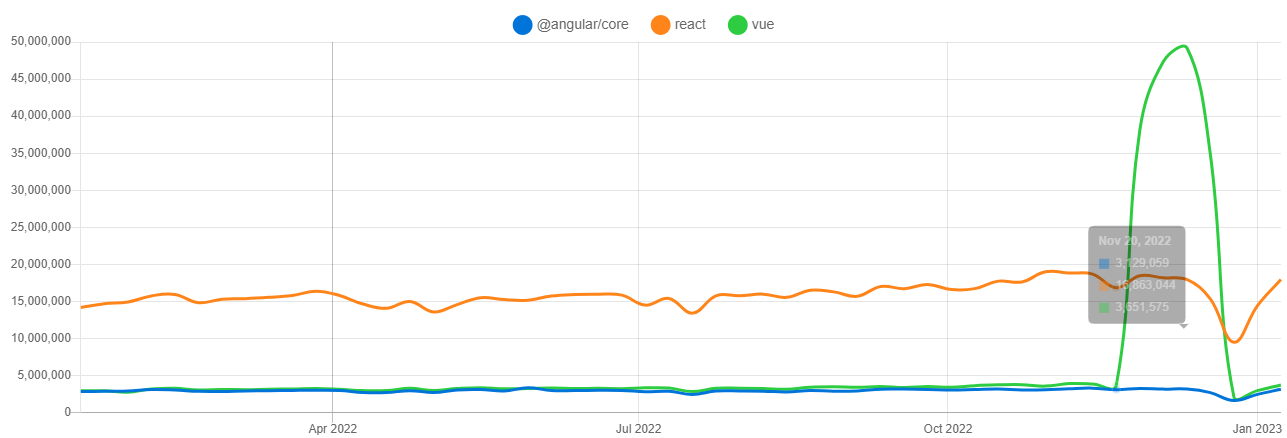
\includegraphics[width=.75\textwidth]{figures/technical/frontendFrameworks.png}
    \caption{Vergleich Downloadzahlen verschiedener Frontend Frameworks \cite{npm2023}}
    \label{fig:downloadFrontendFrameworks}
  \end{centering}
\end{figure}

\section{Material-UI}
\label{sec:material-ui}

Material-UI (kurz \gls{mui}) ist eine Bibliothek, die es ermöglicht, Komponenten aus dem Material Design zu verwenden.
Diese Komponenten sind konfigurierbar und können so an die eigenen Bedürfnisse angepasst werden.
Trotzdem entsprechen Sie alle einer einheitlichen Designsprache, die von Google entwickelt wurde. \footnote{Vgl. Google 2021 \cite{google2021}}

MUI bietet Komponenten für folgende Bereiche an:

\begin{itemize}
  \item \textbf{Navigation} – Komponenten für die Navigation.
  \item \textbf{Inputs} – Komponenten für die Eingabe von Daten.
  \item \textbf{Layout} – Komponenten für das Layout der Website.
  \item \textbf{Data Display} – Komponenten für die Anzeige von Daten.
  \item \textbf{Feedback} – Komponenten für die Rückmeldung an den Benutzer.
  \item \textbf{Surfaces} – Komponenten für Oberflächen.
  \item \textbf{Utils} – Komponenten für die Unterstützung.
\end{itemize}

Diese Bibliothek wird von Material-UI SAS. entwickelt und ist Open-Source auf Github verfügbar.
MUI bietet eine direkte Integration mit React. \footnote{Vgl. Material-UI 2022 \cite{mui2022}}

\subsection{Einsatz im Projekt}
\label{sub:material-uiUsage}

Da React nur sehr rudimentäre Komponenten für die Benutzeroberfläche bereitstellt, wurde MUI verwendet, um die Benutzeroberfläche zu gestalten.
Es bietet eine große Auswahl an Komponenten, die direkt in React verwendet werden können.

\subsection{Grund für Technologieentscheidung}
\label{sub:material-uiReason}

MUI vereinfachte die Gestaltung der Benutzeroberfläche, da es eine große Auswahl an Komponenten bietet, die direkt in React verwendet werden können.
Aus diesem Grund konnten die Entwickler schnell mit der Gestaltung der Benutzeroberfläche beginnen.

\section{Firebase}
\label{sec:firebase}

Firebase ist eine \gls{baas} Plattform, die die Bereitstellung von Backend-Funktionalität ermöglicht inklusive Datenbank, Authentifizierung, Datei-Upload, etc.
Dabei wird die Funktionalität in einzelne Module aufgeteilt, die unabhängig voneinander verwendet werden können.
Die Plattform wird von Google entwickelt\footnote{Vgl. Firebase 2022 \cite{firebase2022}} und besteht aus mehreren Komponenten, die nun kurz vorgestellt werden.

\subsection{Firebase Authentication}
\label{sub:firebase-authentication}

Firebase Authentication ist ein Modul von Firebase, das die Authentifizierung von Nutzern ermöglicht.
Dabei werden verschiedene Authentifizierungsmethoden unterstützt, wie z. B. E-Mail und Passwort, Google, Facebook, etc.
Außerdem ist es möglich eigene Authentifizierungsmethoden zu implementieren, sowie Nutzer über Telefonnummern zu authentifizieren.
Dabei können Nutzer auch in mehreren Geräten gleichzeitig eingeloggt sein.

Bis auf die Authentifizierungsmethode über Telefonnummern, die nur in den USA verfügbar ist, werden alle Authentifizierungsmethoden kostenlos angeboten. \footnote{Vgl. Firebase Authentication 2022 \cite{authentication2022}}

\subsection{Firebase Realtime Database}
\label{sub:firebase-realtime-database}

Firebase Realtime Database ist ein Modul von Firebase, das die Bereitstellung einer Datenbank ermöglicht.
Diese Datenbank ist eine NoSQL Datenbank, ähnlich wie MongoDB.
Hier werden die Daten nicht relational in Dokumenten gespeichert, sondern in einer Baumstruktur.
Updates in der Datenbank werden in Echtzeit an alle Nutzer gesendet, die sich mit der Datenbank verbinden.\footnote{Vgl. Firebase Realtime Database 2022 \cite{realtimedatabase2022}}

\subsection{Firebase Cloud Firestore}
\label{sub:firebase-cloud-firestore}

Firebase Cloud Firestore ist ein Modul von Firebase, das die Bereitstellung einer Datenbank ermöglicht.
Dabei wird die Datenbank in einzelne Dokumente aufgeteilt, die in einer Baumstruktur organisiert sind.
Firestore ist die Weiterentwicklung der Realtime Database und bietet einige Vorteile gegenüber dieser.
So ist die Datenbank in mehrere Regionen aufgeteilt, was die Verfügbarkeit erhöht.
Außerdem ist es möglich, die Datenbank in mehrere Projekte aufzuteilen, was die Sicherheit erhöht.
Abfragen in der Datenbank können mit Indexen optimiert werden, was die Performance verbessert. \footnote{Vgl. Firebase Cloud Firestore 2022 \cite{firestore2022}}

\subsection{Firebase Storage}
\label{sub:firebase-storage}

Firebase Storage ist ein Modul von Firebase, das die Bereitstellung von Datei-Upload ermöglicht.
Dabei können Dateien in einem Bucket gespeichert werden, das in einzelne Ordner aufgeteilt ist.
Der Datei-Upload kann über die Firebase Konsole oder über die Firebase SDK’s erfolgen.
Diese Funktion ist vergleichbar mit AWS S3 Buckets.\footnote{Vgl. Firebase Storage 2022 \cite{cloudstorage2022}}

\subsection{Einsatz im Projekt}
\label{sub:firebase-use}
Firebase wurde im Projekt für die Bereitstellung der Datenbank und der Authentifizierung verwendet.
Außerdem speichert es die Bilder, die von den Nutzern hochgeladen werden.


\subsection{Grund für Technologieentscheidung}
\label{sub:firebase-reason}
Durch Firebase konnte die Entwicklung der Backend-Funktionalität beschleunigt werden, da die Entwickler sich nicht um die Bereitstellung dieser Funktionalität kümmern mussten.

\section{Github}
\label{sec:github}

Github ist eine Plattform, die es ermöglicht, Softwareprojekte zu verwalten.
Diese Plattform wird von Github Inc. entwickelt. Github bietet eine direkte Integration mit Git.
Die wichtigsten Funktionen von Github sind in Tabelle \ref{tab:github} aufgeführt.\footnote{Vgl. Github 2022 \cite{github2022}}

\begin{table}[ht]
  \begin{tabularx}{\textwidth}{|l|X|}
  \hline
  \textbf{Funktion} & \textbf{Beschreibung} \\ \hline
  Versionsverwaltung & Github bietet Versionsverwaltung auf Grundlage von Git an. \\ \hline
  Projektmanagement & Anforderungen können als Issues angelegt und verwaltet werden. \\ \hline
  Dokumentation & Mithilfe von Markdown Wikis. \\ \hline
  Teamarbeit & In Form von Kommentaren, Reviews, etc. \\ \hline
  Hosting & Bereitstellung statischer Seiten. \\ \hline
  \gls{ci}/\gls{cd} & Automatisierte Tests und Deployment. \\ \hline
  \end{tabularx}
  \caption{Funktionen von Github}
  \label{tab:github}
\end{table}

\subsection{Einsatz im Projekt}
\label{sub:github-use}

Github wurde im Projekt für die Versionsverwaltung und \gls{ci} verwendet.
Die Versionsverwaltung wurde durch die Integration mit Git ermöglicht.
Außerdem wurden Github Actions benutzt, welches automatisierte Tests und andere Sanity-Checks ermöglicht.

\subsection{Grund für Technologieentscheidung}
\label{sub:github-reason}

Github wurde im Projekt eingesetzt, da es eine gute Integration mit Git bietet und somit die Versionsverwaltung vereinfacht.
Außerdem wurde durch die verfügbare \gls{ci} Funktionalität die Qualität des Codes verbessert und stetig getestet werden.
Die Entwicklungsgeschwindigkeit wurde dadurch vereinfacht.

\section{Vercel}
\label{sec:vercel}

Vercel ist eine Hosting-Plattform, die es ermöglicht, statische Webseiten zu hosten.
Diese Plattform wird von Vercel Inc. entwickelt.
Vercel bietet eine direkte zu \ref{sec:github} und erstellt neue Deployments und Builds, sobald ein neuer Commit in Github verfügbar ist.
Dies funktioniert auch mit mehreren Branches und Pull Requests. Jedes Deployment wird mit einer eigenen URL versehen, sodass mehrere Versionen der gleichen Webseite gleichzeitig verfügbar sind.
So können Pull Requests getestet werden, bevor sie in den Master Branch gemerged werden.\footnote{Vgl. Vercel 2022 \cite{vercel2022}}

\subsection{Einsatz im Projekt}
\label{sub:vercel-use}

Vercel wurde im Projekt für die Bereitstellung der Webanwendung verwendet.
Sobald bei Github ein neuer Commit verfügbar ist, wird automatisch ein neues Deployment erstellt.
Dies geschah für den main-Branch auf der Domain \url{https://dahoam.roser.dev} und für den dev-Branch auf der Domain \url{https://dev.dahoam.roser.dev}.
Jeder andere Branch bekam sein eigenes Deployment auf einer eigenen Domain, welche von Vercel erstellt wurde.

\subsection{Grund für Technologieentscheidung}
\label{sub:vercel-reason}

Vercel wurde verwendet, um die Bereitstellung der Webanwendung zu vereinfachen.
Nach Errichtung des Github Repositories und initialer Projekterstellung wurde die Integration mit Vercel in wenigen Klicks aktiviert und hostet seitdem kostenlos die Webanwendung.

\clearpage
\section{Jira}
\label{sec:jira}

Jira ist eine Plattform, die es ermöglicht, Softwareprojekte zu verwalten.
Diese Plattform wird von Atlassian entwickelt.

Die wichtigsten Funktionen von Jira sind in Tabelle \ref{tab:jira} aufgeführt.\footnote{Vgl. Atlassian 2023 \cite{attlassian2023}}

\begin{table}[ht]
  \begin{tabularx}{\textwidth}{|l|X|}
  \hline
  \textbf{Funktion} & \textbf{Beschreibung} \\ \hline
  Projektmanagement & Anforderungen können als Issues angelegt und verwaltet werden. \\ \hline
  Dokumentation & Mithilfe von Markdown Wikis. \\ \hline
  Teamarbeit & In Form von Kommentaren, Reviews, etc. \\ \hline
  \end{tabularx}
  \caption{Funktionen von Jira}
  \label{tab:jira}
\end{table}

\subsection{Einsatz im Projekt}
\label{sub:jira-use}

In Jira wurden die einzelnen User Stories verwaltet und bearbeitet, sowie in Sprints eingeplant.
Durch ein Kanbanboard wurden die einzelnen User Stories in den einzelnen Sprints angezeigt.
Jira bietet eine direkte Integration mit Github.

\subsection{Grund für Technologieentscheidung}
\label{sub:jira-reason}

Jira wurde verwendet, um die Verwaltung der User Stories zu vereinfachen.
Durch die direkte Integration mit Github wurden die einzelnen User Stories mit den dazugehörigen Commits verknüpft.
Dadurch konnte die Entwicklung der einzelnen User Stories nachvollzogen werden.
Außerdem ist es ein sehr simples Tool, welches für die Verwaltung von User Stories sehr gut geeignet ist.
